\section{Triển khai thuật toán}
Toàn bộ code của thuật toán có thể tìm được ở link sau.
\href{https://github.com/tincuri/BTL_pptinh}{https://github.com/tincuri/BTL\_pptinh}
\subsection{Tam giác hóa}
Ở bước này nhóm em sử dụng thuật toán của ông Seidel\cite{} lấy source code từ trang web sau \cite[]. Ông ấy hình thang hóa đa giác và từ đó tách đa giác đó ra thành các monotone polygon. Từ đây ông dùng một thuật toán tham lam để tam giác hóa các đa giác con này. Độ phức tạp của thuật toán hình thang hóa là $O(n \text{log*}n)$ , với log* n là hàm log lặp\footnote{Từ nguyên: iterative logarithm} của n với tốc độ biến thiên rất chậm $\log_b^* (n) << \log_b(n)$ và trong thực tế thì gần tương đương với hàm hằng. Phần tam giác hóa của các monotone polygon con có độ phức tạp $O(n)$. Do đó độ phức tạp của thuật toán tam giác hóa là  $O(n \text{log*}n)$.
\subsection{Dual tree}
Ở phần này nhóm em sử dụng cấu trúc \textbf{Doubly connected edge list (dcel)} để biểu diễn hình dạng của đa giác đã được tam giác hóa.

Dcel là một kiểu dữ liệu dùng để biểu diễn một đồ thị phẳng $G(V,E)$ với $V=\{v_1,v_2,..v_n\}$ là là tập hợp các điểm của đồ thị và $E=\{e_1, e_2, ..e_n\}$ là tập hợp các cạnh kết nối giữa các điểm. 
dcel gồm 3 kiểu dữ liệu: half\_edge, vertex, face.  \textit{ half\_edge} như tên gọi của nó, là một cấu trúc dữ liệu gần giống như một nửa của một cạnh. Mỗi \textit{half\_edge} chứa các miền dữ liệu sau.
\begin{itemize}
  \item Twin, là một cạnh đối ngược với nó.
  \item Origin, là điểm bắt đầu của \textit{half\_edge}.
  \item Next, là một \textit{half\_edge} có điểm bắt đầu là điểm kết thúc của \textit{half\_edge} này.
  \item Prev, là một \textit{half\_edge} có điểm kết thúc là điểm bắt đầu của \textit{half\_edge} này.
  \item IncidentFace, là một \textit{face} mà có \textit{half\_edge} này làm bờ.
\end{itemize}

\textit{face} và \textit{vertex} có thêm một miền dữ liệu chứa một \textit{half\_edge} mà các dữ liệu đó kề.

Các miền dữ liệu của \textit{half\_edge} được diễn tả như hình sau.
\begin{figure}[h]
  \centering
  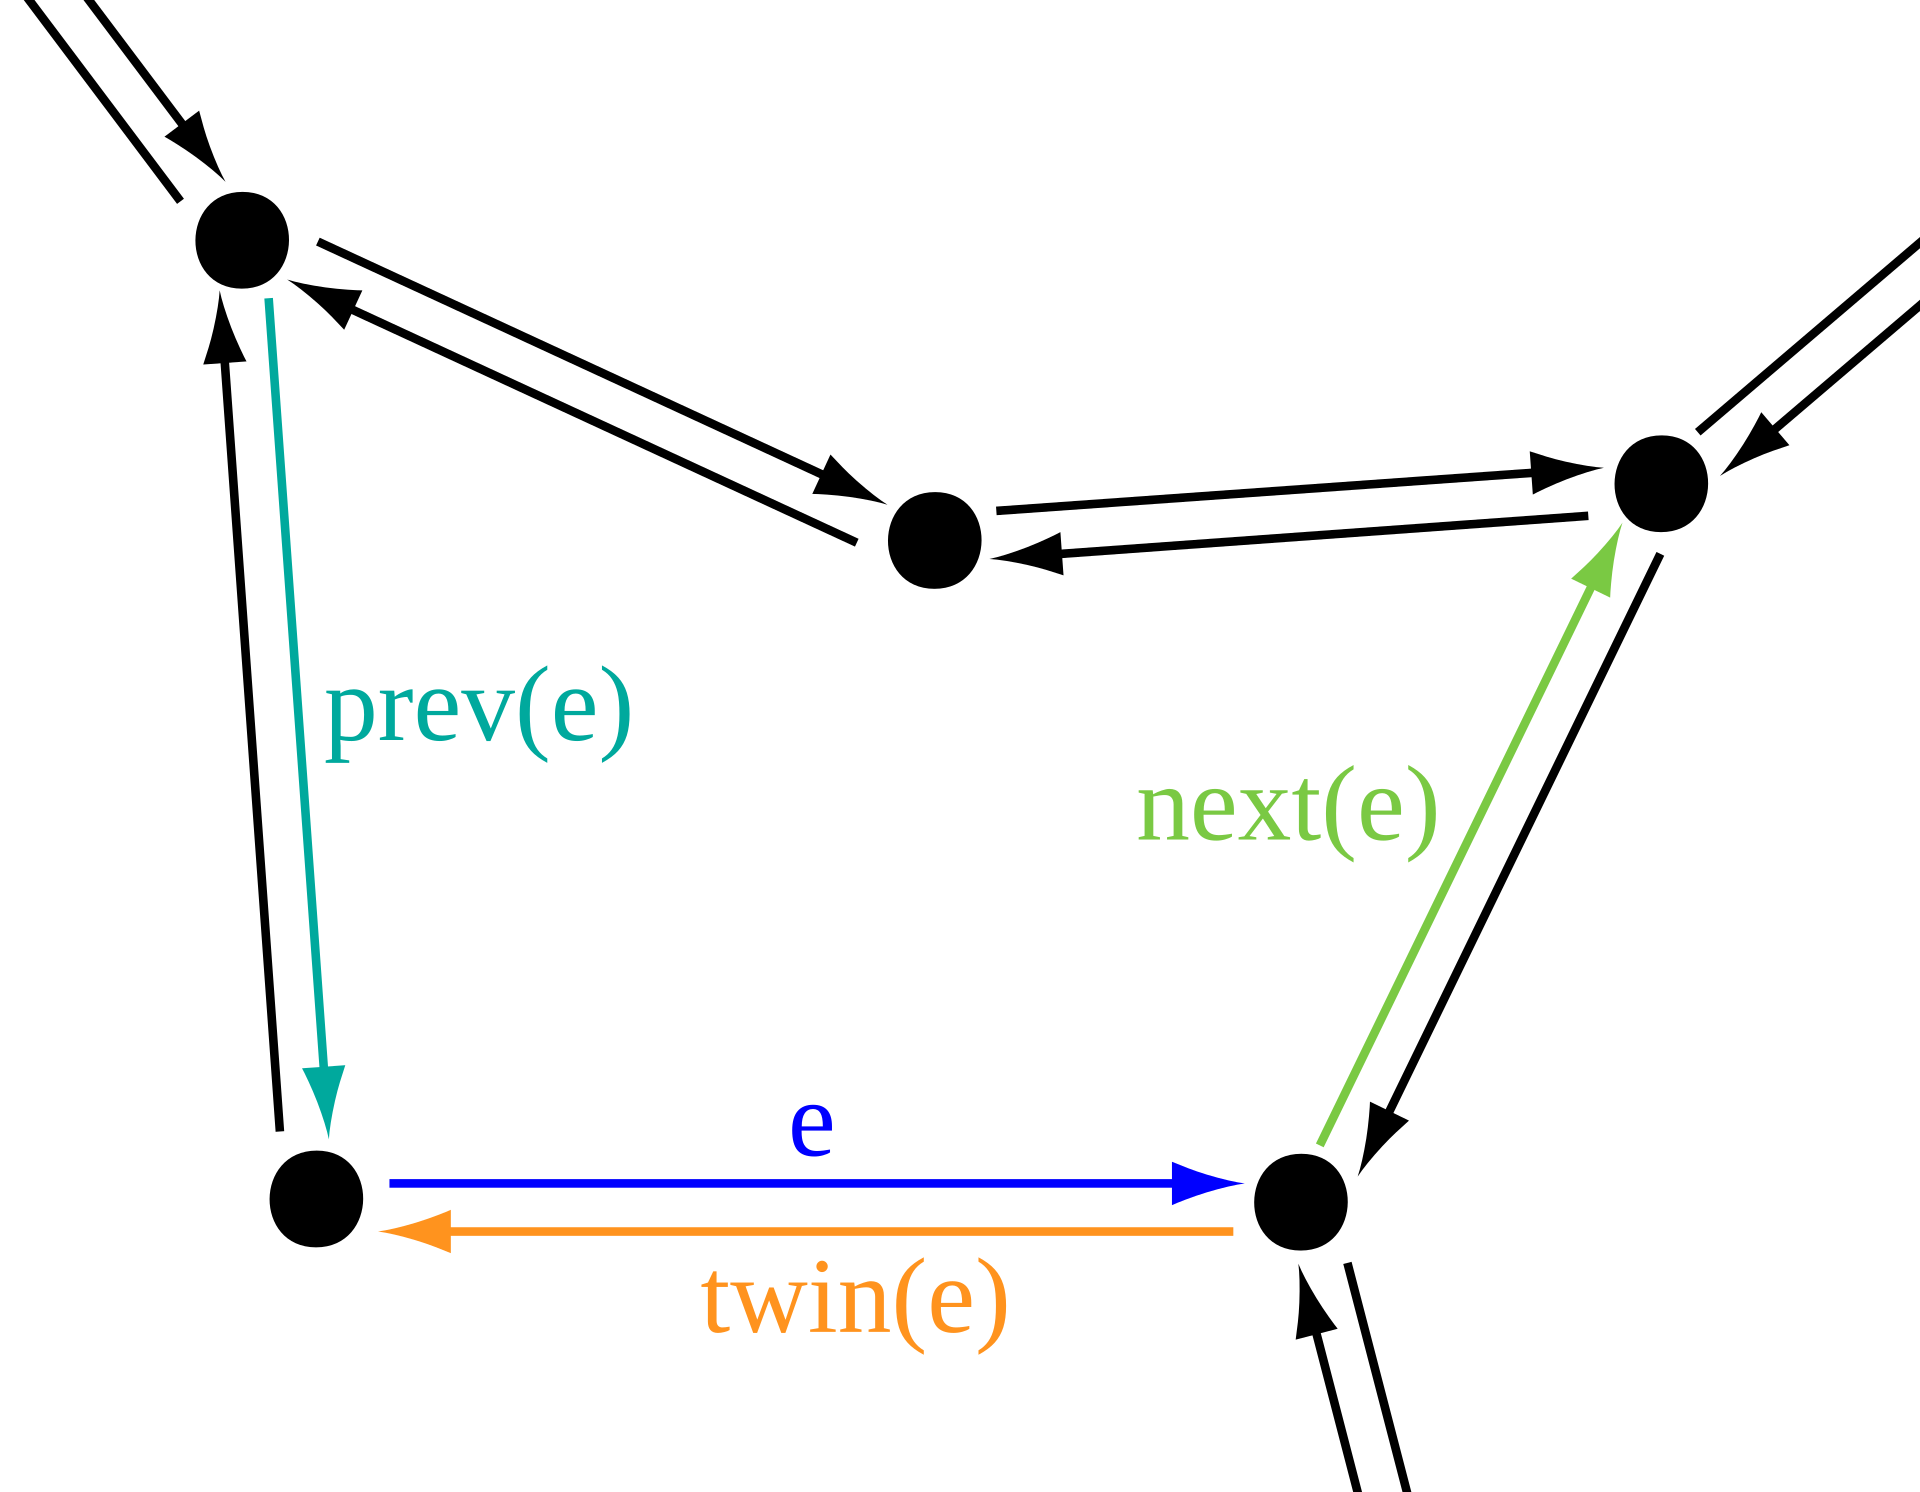
\includegraphics[width=0.45\textwidth]{Images/Dcel-halfedge-connectivity.svg.png}
\end{figure}

Dcel có thể được dựng dễ dàng như sau\cite{dcel}:
\begin{enumerate}
    \item Với từng điểm $v_i$ tạo một \textit{vertex} tương ứng.
    \item Với từng cạnh $e_i$ tạo hai \textit{half\_edge} tương ứng, đặt Origin cho 2 \textit{half\_edge} đó.
    \item Với từng \textit{vertex}, Sắp xếp các cạnh có nó là Origin theo chiều kim đồng hồ.
    \item Với hai \textit{half\_edge} $e_1, e_2$ kề nhau (trong thứ tự đã sắp xếp của một \textit{vertex} ở bước 3), gán $\text{Next}(\text{Twin}(e_1)) = e_2$ và $\text{Prev}(e_2) = \text{Twin}(e_1)$. 
    \item Lần lượt gán một \textit{face} cho các chuỗi \textit{half\_edge}
\end{enumerate}
Trong bước cuối, ta có thể lợi dụng việc gán mặt để tạo cho từ mặt một đỉnh trong đồ thị, và liên kết các đỉnh lại với nhau nếu hai mặt có chung một cạnh, mỗi liên kết có một miền dữ liệu là cạnh liên kết giữa hai mặt. Do đó ta có thể dựng được Dual tree của đa giác khi đang dựng dcel.

Như ta đã biết, để tam giác hóa một đa giác $n$ cạnh thì ta cần thêm $n-3$ đường chéo, mà mỗi đường chéo có 2 đỉnh. Do đó, trong trường hợp trung bình, mỗi đỉnh sẽ liên kết với khoảng 4 cạnh (thêm hai cạnh của đa giác ban đầu). Vì vậy độ phức tạp trung bình của thuật toán tạo DCEL trong trường hợp tam giác hóa là $O(n)$ nếu như bảo đảm các góc có số lượng cạnh liên kết tới nó gần ngang nhau. Trong trường hợp tệ nhất, tất cả các cạnh đều liên kết tới một góc, độ phức tạp của thuật toán khi này là $O(n\log n)$ do bước sắp xếp có độ phức tạp là $O(n\log n)$.
\subsection{Sleeve}
Bước đầu tiên, ta cần tìm vị trí của 2 điểm cần xét, ta có thể check\footnote{} xem điểm có nằm trong một tam giác bằng định hướng của nó với 3 đỉnh tam giác. Ta chỉ cần lặp qua các \textit{face} đến khi nào tìm được \textit{face} mà điểm đó nằm trong. Thuật toán có độ phức tạp là $O(n)$.

Với Dual Tree đã được tạo như trên, Nhóm em sử dụng Depth-first search (DFS) để tìm đường liên kết giữa 2 đỉnh tương ứng với 2 tam giác chứa 2 điểm. Đây chính là \textit{sleeve}. Từ đây ta rút ra được các đường chéo cần xét từ các liên kết. Độ phức tạp của DFS là $O(V+E)$ với $V = n$ là số đỉnh còn $E = n - 3$ là số cạnh. Do đó trong trường hợp này thuật toán tạo \textit{sleeve} có độ phức tạp là $O(n)$.

\subsection{Lee \& Preparata}
% hello ldm
% tui moi update anh vo latex de m can thi chen` vo result or smth
% oyasumi


\subsection{Kết quả}

\subsubsection{Độ phức tạp của các thuật toán}

\begin{table}[h]
    \centering
    \begin{tabular}{|c|c|c|}
    \hline
        \textbf{Thuật toán} & \textbf{Độ phức tạp trung bình}  & \textbf{Độ phức tạp tệ nhất}\\
    \hline
        Tam giác hóa & $O(n\text{log*}n)$ & $O(n\text{log*}n)$\\
    \hline
        Tìm Dual Tree & $O(n)$ & $O(n\log(n))$\\
    \hline
        Tìm Sleeve & $O(n)$ & $O(n)$ \\
    \hline
        Lee \& Preparata & $O(n)$ & $O(n)$\\
    \hline
    \end{tabular}
    \caption{Độ phức tạp của các thuật toán}
    \label{tab:complexity}

\subsubsection{Thời gian chạy thực tế}
\end{table}
